% OptimalBids.jl: a market is four functions, and one market object gives three
% kinds of access to the profit of an offer.
%
% build_market sets the market up once. For each offer u, change_bids! writes the
% offered quantities into the network, clear_market! solves the operator's
% clearing (a PowerModels OPF), and calculate_profit reads the cleared quantities
% q* and bus prices pi* of the strategic generators. The same object is then
% evaluated (profit_for_bid!), given a price-based first-order estimate
% (profit_and_gradient_for_bid!), or written into the lower level of a bilevel
% model (instantiate_model). No loop is drawn: the package evaluates u -> J(u);
% the search over u belongs to whichever optimizer calls it.
% Notation follows docs/src/index.md ("Notation").
%
% Build: make -C docs/src/assets/diagrams/src
%   pdflatex market.tex                                    -> wide layout
%   pdflatex -jobname=optimalbids--market-compact market.tex -> narrow layout
\documentclass[tikz,border=4pt]{standalone}
\usepackage{amsmath,amssymb,bm}
\usepackage[T1]{fontenc}
\usepackage[scaled=0.92]{helvet}
\usepackage[scaled=0.95]{zi4}
\renewcommand{\familydefault}{\sfdefault}
\usetikzlibrary{arrows.meta,shapes.geometric,shapes.symbols,calc,positioning}

% palette of the TS-DDR figure
\definecolor{dTeal}{HTML}{1A9AA0}
\definecolor{dTealLine}{HTML}{3FB3B8}
\definecolor{dNavy}{HTML}{3F4C8C}
\definecolor{dInk}{HTML}{1E2235}
\definecolor{dRed}{HTML}{E4573D}
\definecolor{dCoral}{HTML}{E2765A}
\definecolor{dOrange}{HTML}{F4A93B}
\definecolor{dPeach}{HTML}{FBD9AC}
\definecolor{dPanel}{HTML}{EEF0F2}
\definecolor{dGray}{HTML}{8A90A0}
\definecolor{dShadow}{HTML}{D5DAE3}

\newif\ifcompact
\edef\compactname{\detokenize{optimalbids--market-compact}}
\edef\jobstr{\jobname}
\ifx\jobstr\compactname\compacttrue\fi

\tikzset{
  >={Stealth[length=5pt,width=4pt]},
  every node/.style={text=dInk},
  title/.style={anchor=west,font=\normalsize,inner sep=0pt},
  head/.style={font=\normalsize\bfseries,text=dNavy,anchor=west},
  note/.style={font=\itshape\small,text=dNavy,anchor=west},
  dia/.style={diamond,fill=dOrange,draw=none,minimum size=0.95cm,inner sep=0pt,aspect=1,
              font=\normalsize},
  card/.style={rectangle,rounded corners=4pt,fill=white,draw=dShadow,line width=0.6pt},
  chip/.style={rectangle,rounded corners=3pt,fill=dPanel,draw=none,font=\small\ttfamily,
               inner xsep=4pt,inner ysep=3pt},
  fwd/.style={->,dTealLine,line width=0.9pt},
  wout/.style={->,dOrange,line width=0.9pt},
}

% Lane frame in the paper style: two shadow copies behind a teal rounded frame.
\newcommand{\lane}[4]{% #1 x0, #2 y0, #3 x1, #4 y1
  \foreach \o/\c in {0.16/dShadow!60,0.08/dShadow}
    \draw[\c,fill=white,rounded corners=5pt,line width=0.6pt]
      (#1+\o,#2-\o) rectangle (#3+\o,#4-\o);
  \draw[dTealLine,fill=white,rounded corners=5pt,line width=0.9pt] (#1,#2) rectangle (#3,#4);}

% The operator's clearing (the follower's problem).
\newcommand{\clearing}{%
  $\begin{aligned}
    \min_{\mathbf g}\;\; & \textstyle\sum_{j} c_j\,g_j\\[1pt]
    \text{s.t.}\;\; & \text{power flow, balance at bus } n\;:\;\pi_n\\[1pt]
    & 0\le g_i\le u_i,\quad i\in\mathcal S
  \end{aligned}$}
\newcommand{\profit}{$J(u)=\sum_{i\in\mathcal S} q_i^\star(u)\,\pi_i^\star(u)$}

% The three kinds of access. #1 = top-left corner of the block.
\newcommand{\access}[1]{\begin{scope}[shift={(#1)}]
  \node[head] at (0,0) {Evaluation};
  \node[chip,anchor=west] at (0,-0.55) {profit\_for\_bid!(market, u)};
  \node[note] at (0,-1.08) {$J(u)$, one clearing per call};
  \node[head] at (0,-1.75) {Local};
  \node[chip,anchor=west] at (0,-2.3) {profit\_and\_gradient\_for\_bid!};
  \node[anchor=west] at (0,-2.88) {$\partial J/\partial u_i\approx\pi_i^\star$ if $q_i^\star\approx u_i$, else $0$};
  \node[note] at (0,-3.38) {prices held fixed; also a ChainRules rule};
  \node[head] at (0,-4.05) {Exact};
  \node[chip,anchor=west] at (0,-4.6) {instantiate\_model(market; jump\_model)};
  \node[note] at (0,-5.13) {the clearing as the lower level of a bilevel model};
\end{scope}}

% Inside the clearing card, under a rule: what solves it.
\newcommand{\solver}[1]{% #1 = left point of the row
  \node[chip,anchor=west] at (#1) {clear\_market!};
  \node[note] at ($(#1)+(2.35,0)$) {PowerModels OPF: DC, AC, \dots};}

\begin{document}
\ifcompact
% ============================ narrow (phone) layout ============================
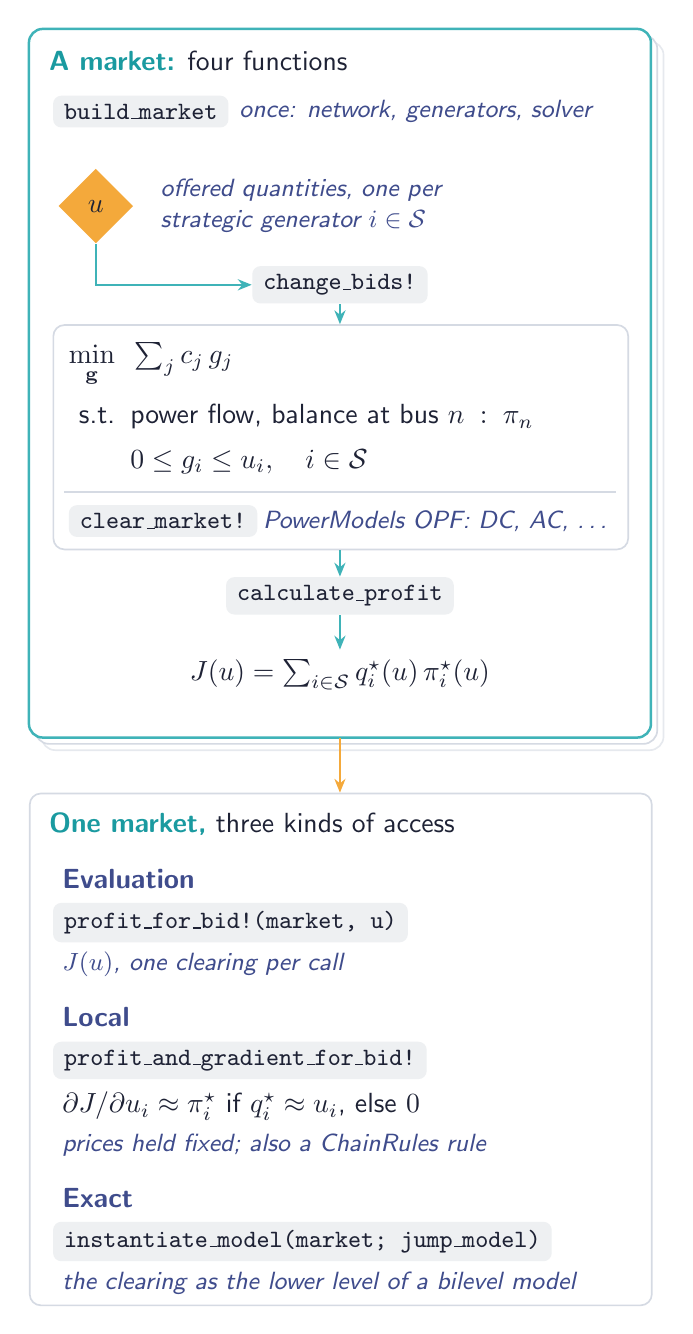
\begin{tikzpicture}
  \lane{0}{6.5}{7.9}{15.5}
  \node[title] at (0.25,15.1) {\textcolor{dTeal}{\bfseries A market:} four functions};
  \node[chip,anchor=west] at (0.3,14.45) {build\_market};
  \node[note] at (2.55,14.45) {once: network, generators, solver};
  \node[dia] (u) at (0.85,13.25) {$u$};
  \node[note] at (1.55,13.45) {offered quantities, one per};
  \node[note] at (1.55,13.05) {strategic generator $i\in\mathcal S$};
  \node[chip] (cb) at (3.95,12.25) {change\_bids!};
  \draw[fwd] (u.south) |- (cb.west);
  \node[card,minimum width=7.3cm,minimum height=2.85cm,anchor=north west] (clr) at (0.3,11.75) {};
  \draw[fwd] (cb.south) -- (cb.south |- clr.north);
  \node[anchor=north west,inner sep=0pt] at (0.5,11.55) {\clearing};
  \draw[dShadow,line width=0.6pt] (0.45,9.62) -- (7.45,9.62);
  \solver{0.5,9.25}
  \node[chip] (cp) at (3.95,8.3) {calculate\_profit};
  \draw[fwd] (cb.south |- clr.south) -- (cp.north);
  \node (J) at (3.95,7.3) {\profit};
  \draw[fwd] (cp.south) -- (J.north);

  \draw[wout] (3.95,6.5) -- (3.95,5.8);
  \node[card,minimum width=7.9cm,minimum height=6.5cm,anchor=north west] at (0,5.8) {};
  \node[title] at (0.25,5.4) {\textcolor{dTeal}{\bfseries One market,} three kinds of access};
  \access{0.3,4.7}
\end{tikzpicture}
\else
% =============================== wide layout ===================================
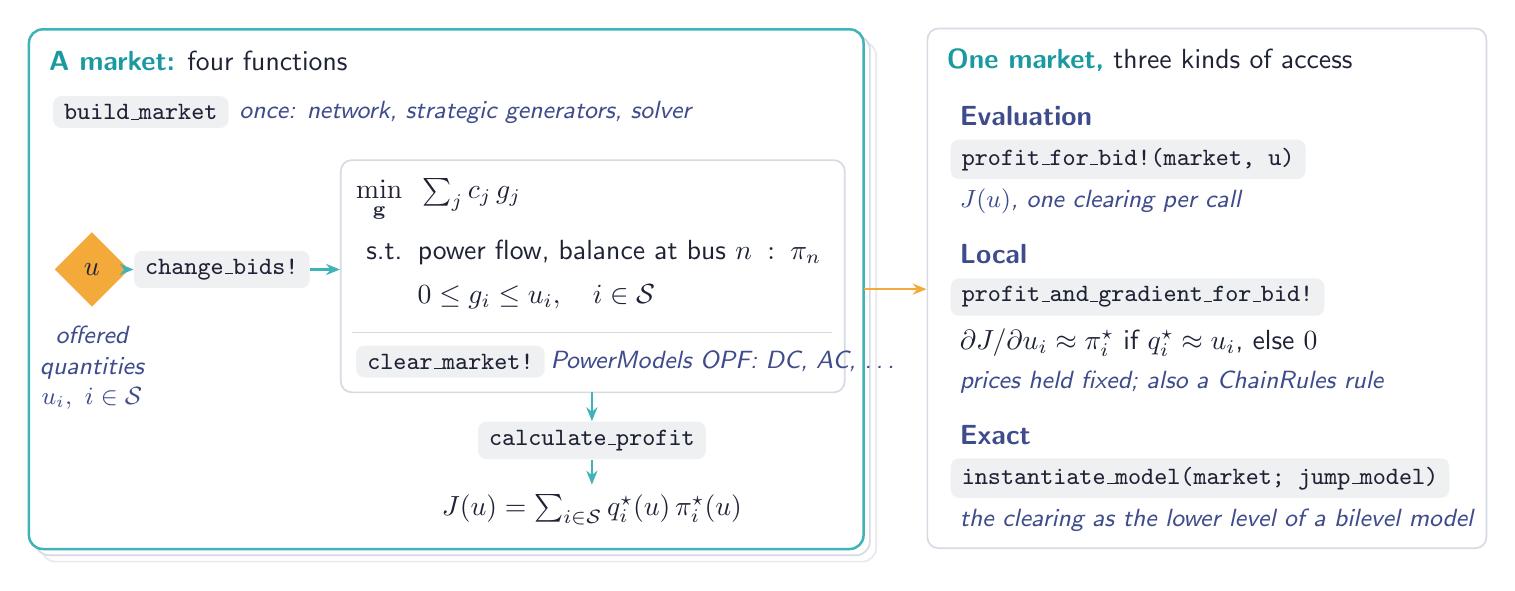
\begin{tikzpicture}
  \lane{0}{0}{10.6}{6.6}
  \node[title] at (0.25,6.2) {\textcolor{dTeal}{\bfseries A market:} \textcolor{dInk}{four functions}};
  \node[chip,anchor=west] at (0.3,5.55) {build\_market};
  \node[note] at (2.55,5.55) {once: network, strategic generators, solver};
  % offer
  \node[dia] (u) at (0.8,3.55) {$u$};
  \node[note,anchor=north,align=center] at (0.8,2.95) {offered\\quantities\\$u_i,\ i\in\mathcal S$};
  % clearing
  \node[card,minimum width=6.4cm,minimum height=2.95cm,anchor=north west] (clr) at (3.95,4.95) {};
  \node[anchor=north west,inner sep=0pt] at (4.15,4.75) {\clearing};
  \draw[dShadow,line width=0.6pt] (4.1,2.75) -- (10.2,2.75);
  \solver{4.15,2.38}
  \node[chip] (cb) at (2.45,3.55) {change\_bids!};
  \draw[fwd] (u.east) -- (cb.west);
  \draw[fwd] (cb.east) -- (cb.east -| clr.west);
  % profit
  \node[chip] (cp) at (7.15,1.38) {calculate\_profit};
  \draw[fwd] (7.15,2.0) -- (cp.north);
  \node (J) at (7.15,0.5) {\profit};
  \draw[fwd] (cp.south) -- (J.north);

  \draw[wout] (10.6,3.3) -- (11.4,3.3);
  \node[card,minimum width=7.1cm,minimum height=6.6cm,anchor=south west] at (11.4,0) {};
  \node[title] at (11.65,6.2) {\textcolor{dTeal}{\bfseries One market,} \textcolor{dInk}{three kinds of access}};
  \access{11.7,5.5}
\end{tikzpicture}
\fi
\end{document}
